\documentclass{myReport}
%%%%%%%%%%%%%%%%%%%%%%%%%%%%%%%%%%%%%%%%%%%%%%%%%%%%%%%%%%%%%%%%%%%%%%
%Packages
\usepackage{xcolor}
\usepackage{enumitem}
\usepackage{float}
\usepackage{wrapfig}
\usepackage{sidecap}
\usepackage{caption}
\usepackage{abstract}
\usepackage{setspace}
\usepackage{myStyle}
\usepackage[utf8]{inputenc}
\usepackage[french]{babel} %to change language
\usepackage{amsmath, amsthm, amsfonts}
\usepackage{graphicx}
% \usepackage{biblatex}
% \addbibresource{references.bib}
\usepackage[footnote]{acronym}
\nocite{*}
%%%%%%%%%%%%%%%%%%%%%%%%%%%%%%%%%%%%%%%%%%%%%%%%%%%%%%%%%%%%%%%%%%%%%%
\newtheorem{theorem}{Theorem}[section]
\newtheorem{corollary}{Corollary}[theorem]
%%%%%%%%%%%%%%%%%%%%%%%%%%%%%%%%%%%%%%%%%%%%%%%%%%%%%%%%%%%%%%%%%%%%%%
\newcommand{\R}{\mathbb{R}}
\newcommand{\cv}[2]{\begin{bmatrix}
    #1\\
    #2\\
\end{bmatrix}}
%%%%%%%%%%%%%%%%%%%%%%%%%%%%%%%%%%%%%%%%%%%%%%%%%%%%%%%%%%%%%%%%%%%%%%
%Doc infos
\title{Introduction to \LaTeX}
%\author{Ahmed IDRISSI\thanks{ENSIAS AI Club}}

%%%%%%%%%%%%%%%%%%%%%%%%%%%%%%%%%%%%%%%%%%%%%%%%%%%%%%%%%%%%%%%%%%%%%%
\setstretch{1.5}
\fontsize{14pt}{18pt}\selectfont
\begin{document}
\students{
    ESSAHIH Abderrahmane
    OUMGHAR Zakaria
}
\supervisors{
    M.ETTALBI Ahmed
}
\jury{

}
\makecoverpage
\newpage

%%%%%%%%%%%%%%%%%%%%%%%%%%%%%%%%%%%%%%%%%%%%%%%%%%%%%%%%%%%%%%%%%%%%%%
\renewcommand{\abstractnamefont}{\normalfont\LARGE\bfseries}
%\renewcommand{\abstracttextfont}{\normalfont\Huge}

\thispagestyle{empty}


%inclusion d'une mage dans le document
\begin{figure}[!h]

\begin{center}
\vspace{2cm}
%taille de l'image en largeur
%remplacer "width" par "height" pour régler la hauteur

\includegraphics[height=4cm]{images/rem1.PNG}
\end{center}
\end{figure}

\hskip7mm



\begin{spacing}{1.3}






\end{spacing}

\begin{figure}[!h]

\begin{center}
\\ [2 cm]
%taille de l'image en largeur
%remplacer "width" par "height" pour régler la hauteur

\includegraphics[height=2cm]{images/rem2.PNG}
\end{center}
\end{figure}
\renewcommand{\abstractname}{\LARGE \bfseries Résumé}
\renewcommand{\abstractnamefont}{\LARGE \bfseries}
\begin{abstract}

 
\vspace{1cm}


\noindent\rule[2pt]{\textwidth}{0.5pt}

{\textbf{Mots clés :}}
\\ 
 
\noindent\rule[2pt]{\textwidth}{0.5pt}
\end{abstract}
\selectlanguage{english}
\renewcommand{\abstractname}{Abstract} 

\begin{abstract}

\vspace{1cm}


\noindent\rule[2pt]{\textwidth}{0.5pt}

{\textbf{Keywords :}}
\\ 
 
\noindent\rule[2pt]{\textwidth}{0.5pt}
\end{abstract}

\newpage
\chapter*{Liste des abréviations}
\begin{acronym}[CP-OFDMX] % Give the longest acronym here

\medskip
\acro{OCI}{\emph{Oracle Cloud Infrastructure}}
\medskip
\acro{UML}{\emph{Unified Modeling Language}}
\end{acronym}
\selectlanguage{french}
\tableofcontents
\listoffigures
%%%%%%%%%%%%%%%%%%%%%%%%%%%%%%%%%%%%%%%%%%%%%%%%%%%%%%%%%%%%%%%%%%%%%%
%\verb|\newline|
%%%%%%%%%%%%%%%%%%%%%%%%%%%%%%%%%%%%%%%%%%%%%%%%%%%%%%%%%%%%%%%%5
\newpage
\ThisLRCornerWallPaper{1}{}
\vspace*{2cm}
\begin{center}
    {\LARGE \textbf{Introduction générale}}
\end{center}
\vspace{2cm}


\newpage
\makeheader
\chapter{Aperçu général et cadre du projet}
% \ThisLRCornerWallPaper{1}{logo/background.png}
% \thispagestyle{empty}
\newpage
\section{Introduction}
Dans ce chapitre, nous présentons le contexte général de notre projet. Nous commencerons par une présentation de la problématique du projet et de ses objectifs. Ensuite, nous élaborerons la partie du déroulement du projet.
\newpage
\section{Présentation du Projet}
Ce projet vise à développer une plateforme centrale pour bien présenter et gérer les départements de l'ENSIAS.

\section{Problématique}
Le site web officiel de l'ENSIAS ne suffit pas pour traduire la qualité de l'école dans le domaine de l'informatique, en particulier en ce qui concerne la visibilité de ce qu'offrent les départements de l'école.

En particulier, il y a un manque de centralisation des données. Les formations des filières sont présentées dans une section du site web actuel qui n'a aucune liaison avec la section des départements, qui ne contient pour le moment que des informations sur les professeurs appartenant à un département spécifique.

D'autre part, la présentation elle-même doit être améliorée pour être plus attrayante. Le design de la plateforme actuelle manque de modernité et des principes simples de l'UX/UI.

\section{Objectifs du projet}
L'objectif principal de notre plateforme est de centraliser les informations concernant les départements de l'ENSIAS, ainsi que de les présenter d'une manière plus moderne et attrayante, attirant ainsi les étudiants, les enseignants et les partenaires possibles. Pour ce faire, nous avons défini les objectifs suivants :
\begin{enumerate}
    \item \textbf{Centraliser la présentation des informations concernant les départements de l'ENSIAS :} Ces informations concernent :
    \begin{itemize}
        \item Les professeurs appartenant à chaque département.
        \item Les chefs des départements de chaque filière.
        \item Les filières disponibles ainsi que les descriptions détaillées de chacune.
        \item Les partenariats académiques (c'est-à-dire les offres de double diplomation, échanges...).
        \item Les ressources appartenant à chaque département (à être détaillées).
    \end{itemize}
    \item \textbf{Être un moyen de gestion des départements :} Cette gestion contiendra des parties comme l'ajout de nouveaux professeurs par les chefs des filières...
    \item Afficher des statistiques afin d'avoir une visualisation plus directe des départements.
\end{enumerate}


\chapter{Analyse et Conception}
% \ThisLRCornerWallPaper{1}{logo/background.png}
% \thispagestyle{empty}
\newpage
\section{Besoins fonctionnels}
\section{Besoins non fonctionnels}





\newpage
\chapter{Réalisation}
% \ThisLRCornerWallPaper{1}{logo/background.png}
% \thispagestyle{empty}
\newpage
% \newpage
% \begin{figure}
%     \centering
%     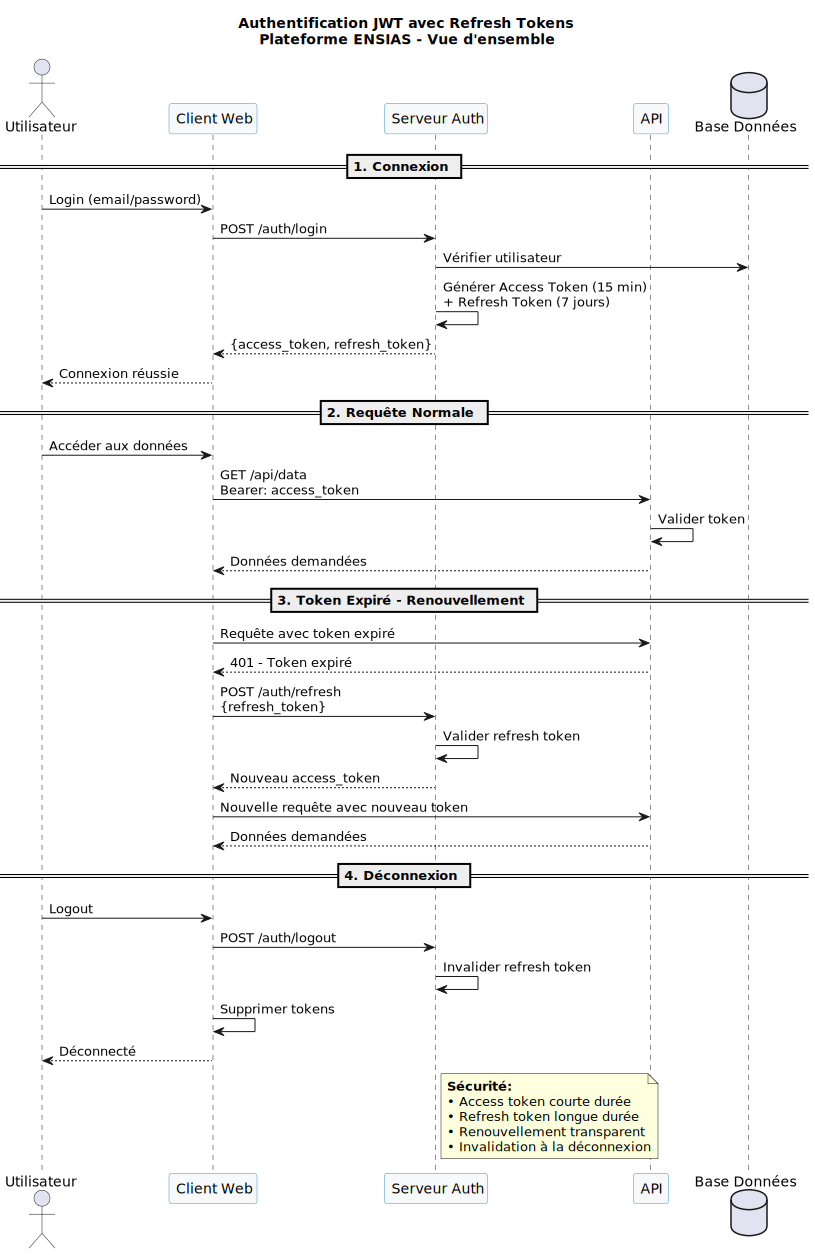
\includegraphics[width=0.5\linewidth]{diagrams/sequence_jwt.svg}
%     \caption{jwt sequence}
%     \label{fig:enter-label}
% \end{figure}

\item \textbf{Spring Boot :} Pour le développement de la partie backend de l'application. Ce framework Java basé sur Spring simplifie grandement la création d'applications robustes, performantes et autonomes. Il facilitera la mise en place rapide d'API RESTful, la gestion de la sécurité (par exemple avec Spring Security) et l'interaction avec la base de données (via Spring Data JPA).

\item \textbf{ReactJS :} Pour la construction de l'interface utilisateur (frontend). Cette bibliothèque JavaScript, maintenue par Facebook, permet de créer des interfaces utilisateur dynamiques et réactives basées sur une architecture de composants. Elle nous aidera à développer une expérience utilisateur moderne et attrayante, conformément aux objectifs du projet.

\item \textbf{PostgreSQL :} Notre système de gestion de base de données relationnelle (SGBDR). PostgreSQL est reconnu pour sa robustesse, sa conformité SQL avancée et ses fonctionnalités d'extensibilité. Il sera utilisé pour stocker et gérer toutes les données de l'application, telles que les informations sur les départements, les professeurs, les formations, les modules, etc., en respectant le modèle entité-relation conçu.

\item \textbf{Docker :} Pour la conteneurisation de notre application. Docker nous permettra d'empaqueter notre application (backend Spring Boot, frontend React servi par un serveur web léger comme Nginx, et potentiellement la base de données PostgreSQL pour l'environnement de développement/test) et ses dépendances dans des conteneurs isolés. Cela garantit la cohérence des environnements entre le développement, les tests et la production, et simplifie grandement le processus de déploiement.

\item \textbf{Oracle Cloud Infrastructure (OCI) / ou autre plateforme Cloud :} Bien que vous ayez mentionné OCI dans la liste des outils, cela se réfère généralement à l'infrastructure d'hébergement. Si OCI est votre cible de déploiement, Docker facilitera le déploiement des conteneurs sur les services de calcul d'OCI (comme Compute Instances ou Oracle Kubernetes Engine - OKE). Si "OCI" se référait à une technologie spécifique liée à Docker (comme Open Container Initiative), alors Docker lui-même est la technologie principale que vous utiliserez pour les conteneurs. Nous utiliserons une plateforme cloud (potentiellement OCI) pour héberger les différents services conteneurisés et rendre l'application accessible.

\item \textbf{Git (et une plateforme comme GitHub/GitLab) :} Pour la gestion de version du code source. Essentiel pour le travail collaboratif, le suivi des modifications, la gestion des branches pour les différentes fonctionnalités et la facilitation de l'intégration continue.
\newpage
\chapter{Réalisation}
% \ThisLRCornerWallPaper{1}{logo/background.png}
% \thispagestyle{empty}
\newpage
\section{Introduction}
Ce chapitre couvre le \textbf{déploiement} de notre solution sur OCI (Oracle Cloud Infrastructure), afin de mettre en évidence la plateforme et de finaliser le projet en le réalisant dans un cycle de bout en bout, de la conception au déploiement.

Ce chapitre détaillera les étapes \textbf{requises} pour ce déploiement.
\newpage
\section{Oracle Cloud Infrastructure}
\subsection{Justification du choix}
Dans le cadre des cours de cloud computing du S3, nous avons eu des comptes OCI. Nous pouvons ainsi utiliser l'un de ces comptes pour obtenir les ressources nécessaires sur le cloud et déployer la plateforme.

\subsection{Étapes du déploiement :}
\subsubsection{Création et configuration d'un réseau cloud virtuel (VCN)}
\subsubsection{Création d'une instance de machine virtuelle sous le VCN}
\subsubsection{Utilisation de Nginx et changements nécessaires pour le déploiement}
\subsubsection{Installation d'un certificat SSL/TLS pour passer en HTTPS}
\subsubsection{Liaison de la VM avec le projet à travers un pipeline CI/CD sous GitHub Actions pour le déploiement continu}
\section{Conclusion}



\chapter{déploiement}
% \ThisLRCornerWallPaper{1}{logo/background.png}
% \thispagestyle{empty}


\newpage



%%%%%%%%%%%%%%%%%%%%%%%%%%%%%%%%%%%%%%%%%%%%%%%%%%%%%%%%%%%%%%%%%%%%%%
\nocite{*} 
\bibliographystyle{plain} 
\renewcommand{\bibname}{Ressources} 
\bibliography{bibliographie} 
\ThisLRCornerWallPaper{1}{logo/background.png}
\thispagestyle{empty}

\end{document}
